% ==================================================================================================================================
% Introduction 

\minitoc  % Affiche la table des matières pour ce chapitre

% ==================================================================================================================================
% Rappels de Topologie

\section{Rappels de Topologie}



% ==================================================================================================================================
% Dérivée Partielles et Différentiabilité

\section{Dérivée Partielles et Différentiabilité}

Le but de ce chapitre est de généraliser les notions de dérivabilités aux fonctions de plusieurs variables. 
Nous nous considérerons des fonctions de la forme $ f : E \longrightarrow F$ où E et F sont des espaces vectoriels normés. 

\begin{remark}[Notations]
    Si $f$ est définie sur une partie de $\R^n$, on dit que $f$ est une \emph{fonction de $n$ variables}.
    \begin{itemize}
        \item si $f : \R^n \longrightarrow \R$ on dit que $f$ est un \emph{champ de scalaires}. 
        \item pour $p \geqslant 2$, la fonction : 
            \[ f : 
                \begin{cases}
                    \R^n \longrightarrow \R^p \\ 
                    (x_1, \dots, x_n) \longmapsto (f_1(x_1), f_2(x_2), \dots, f_n(x_n))
                \end{cases} \] 
            est appelée champ de vecteurs de composantes $f_1, \dots, f_p$. 
            Les composantes $f_i : U \subset \R^n \longrightarrow \R$ sont des fonctions de $n$ variables à valeurs dans $\R$. 
    \end{itemize} 
    Dans ce chapitre, nous nous placerons dans un \emph{ouvert} $U \subset \R^n$. 
\end{remark}

\subsection{Dérivées Partielles}

\begin{definition}[Application Partielle]
    Soit $f : U \subset \R^n \longrightarrow \R^p$ et $a = (a_1, \dots, a_n) \in \U$. 
    Pour tout $ i \in \llbracket 1, n \rrbracket$ on pose : 
        \[ U_i = \{t \in \R \; | \; (a_1, \dots, a_{i-1}, t, a_{i+1,}, \dots, a_n) \in \U\} \] 
    et on définit la i-ème application partielle de $f$ en $a = (a_1, \dots, a_n)$ comme le champ de vecteurs : 
        \[ f_i : 
            \begin{cases}
                U_i \longrightarrow \R^p \\ 
                t \longmapsto f(a_1, \dots, a_{i-1}, t, a_{i+1,}, \dots, a_n)
            \end{cases} \] 
\end{definition}

\begin{definition}[Dérivée Partielle]
    Dans le contexte précédent, $f : \R^n \longrightarrow \R$ admet une i-ème dérivée partielle en $a$. 
    Si $f_i$ est dérivable en $a_i$ et on note alors : 
        \[ \frac{\partial f}{\partial x_i} (a) = f_i'(a_i) \] 
\end{definition}

Le calcul d'une dérivée partielle se ramène donc à un simple de calcul de dérivée (comme une fonction réelle simple). 
Attention à bien dériver en fonction du bon terme. 

\begin{proposition}
    Soit $f : \R^n \longrightarrow \R^p$ un champ de vecteurs de composantes $f_1, \dots, f_p$. 
    $f$ admet une dérivée partielle en $a = (a_1, \dots, a_n)$ par rapport à $x_i$ si chacune de 
    ses composantes en admet une. 
    On note alors : 
        \[ \frac{\partial f}{\partial x_i}(a) = \left(\frac{\partial f_1}{\partial x}(a), \dots, \frac{\partial f_p}{\partial x}(a)\right) \] 
\end{proposition}

\begin{definition}[i-ème dérivée partielle]
    Soit $f : \R^n \longrightarrow \R^p$ un champ de vecteurs de composantes $f_1, \dots, f_p$.
    Si $f$ admet en tout point $a$ de l'ouvert $U$ une ième dérivée partielle, on appelle \emph{i-ème dérivée partielle}
    de $f$ la fonction : 
        \[ \frac{\partial f}{\partial x_i} : 
            \begin{cases}
                U \longrightarrow \R^p \\ 
                a \longmapsto \frac{\partial f}{\partial x_i} (a) 
            \end{cases} \] 
\end{definition}

\begin{definition}[Dérivées Partielles d'ordre supérieur]
    Soit $f : \R^n \longrightarrow \R^p$ et $U$ un ouvert de $\R^n$.
    On définit les dérivées partielles secondes de $f$ comme les dérivées partielles des dérivées partielles de $f$. 
    On peut alors définir par récurrence dérivées partielles d'ordre $p$ de $f$, notées : 
        \[ \frac{\partial ^p f}{\partial x_{i_1} \partial x_{i_2} \dots \partial x_{i_p}} \] 
    comme les dérivées partielles des dérivées partielles d'ordre $p-1$ de $f$. 
\end{definition}

\subsection{Classe $ \mathcal{C}^1$ et Opérations}

Tout comme en analyse réelle, nous pouvons définir les classes de continuité d'un champ de vecteurs. 

\begin{definition}[Classe $ \mathcal{C}^1$]
    Soit $f : \R^n \longrightarrow \R^p$ et $U$ un ouvert de $\R^n$.
    On dit que $f$ est de classe $ \mathcal{C}^1$ si elle admet des dérivées partielles par rapport à toutes ses variables 
    sur $U$ et si elles sont toutes continues sur $U$. 
    On note alors $f \in \mathcal{C}^1(U, \R^p)$. 
\end{definition}

Passons maintenant à quelques propriétés sur les dérivées partielles, analogues à celles vues en analyse réelle. 

\begin{prop}[Dérivées Partielles]
    Soient $f,g \in \mathcal{C}^1(U, \R^p)$ et $ \lambda \in \mathcal{C}^1(U, \R)$.
    Soient $a \in U$ et $ i \in \llbracket 1, n \rrbracket$. 
    On a les propriétés suivantes : 
    \begin{itemize}
        \item \textbf{Somme : } $f+g \in \mathcal{C}^1(U, \R^p)$ et :
            \[ \frac{\partial (f + g)}{\partial x_i} (a) = \frac{\partial f}{\partial x_i}(a) + \frac{\partial g}{\partial x_i}(a) \] 
        \item \textbf{Multiplication : } $ \lambda. f in \mathcal{C}^1(U, \R^p)$ et : 
            \[ \frac{\partial \lambda.f}{\partial x_i} (a) = \lambda(a) . \frac{\partial f}{\partial x_i} (a) + \lambda'(a) . f(a) \] 
        \item Si $\lambda$ ne s'annule pas en $a$, on a : $ \frac{1}{\lambda} \in \mathcal{C}^1(U, \R)$ et : 
            \[ \frac{\partial 1/\lambda}{\partial x_i} (a) = - \frac{1}{\lambda(a)^2} \frac{\partial \lambda}{\partial x_i}(a) \] 
        \item On e déduit donc que si $\lambda$ ne s'annule pas en $a$, on a $\lambda.f \in \mathcal{C}^1(U, \R^p)$ et : 
            \[ \frac{\partial f/\lambda}{\partial x_i}(a) = \frac{1}{\lambda(a)^2} \left(\frac{\partial f}{\partial x_i}(a) . \lambda(a) - f(a) \frac{\partial \lambda}{\partial x_i}(a)\right) \] 
    \end{itemize}
\end{prop}

\begin{proposition}
    On peut déduire des propriétés précédentes que : 
    \begin{enumerate}
        \item Toute application polynomiale est de classe $ \mathcal{C^1}$ sur $\R^n$. 
        \item Toute fraction rationnelle est de classe $ \mathcal{C^1}$ sur son ensemble de définition. 
    \end{enumerate}
\end{proposition}

\subsection{Vecteur Gradient et Matrice Jacobienne}

À partir des définitions précédentes, nous pouvons maintetant nous attaquer aux vecteurs gradients et aux matrices 
Jacobiennes. 

\begin{definition}[Vecteur Gradient]
    Soit $f : U \longrightarrow \R$ un champ de scalaires et $ a \in \U$. 
    Si $f$ admet toutes ses dérivées partielles en $a$, on appelle \emph{vecteur gradient} de $f$ au point $a$ 
    le vecteur de $\R^n$ :
        \[ \boxed{ grad_a(f) = \nabla f = \left(\frac{\partial f}{\partial x_1}(a), \dots, \frac{\partial f}{\partial x_n}(a)\right) } \] 
    Plus généralement, si $f$ admet toutes ses dérivées partielles sur tout $U$ on peut considérer l'application gradient 
    de $f$ : 
        \[ \nabla f : 
            \begin{cases}
                U \subset \R^n \longrightarrow R^n \\ 
                (a_1, \dots, a_n) \longmapsto \nabla f(a) 
            \end{cases} \] 
\end{definition}

\begin{definition}[Matrice Jacobienne]
    Soit $f : U \longrightarrow \R^p, p \leqslant 2$ un champ de vecteurs admettant toutes ses dérivées partielles en $ a \in \U$. 
    On note $f_1, \dots, f_p$ les composantes de $f$. 
    On appelle \emph{matrice jacobienne} de $f$ en $a$, la matrice à $p$ lignes et $n$ colonnes définie par : 
        \[ J_q(f) = 
            \begin{pmatrix}
                \frac{\partial f_1}{\partial x_1}(a) & \frac{\partial f_1}{\partial x_2}(a) & \cdots & \frac{\partial f_1}{\partial x_n}(a) \\ 
                \frac{\partial f_2}{\partial x_1}(a) & \frac{\partial f_2}{\partial x_2}(a) & \cdots & \frac{\partial f_2}{\partial x_n}(a) \\ 
                \vdots & \ddots & \ddots & \vdots \\ 
                \frac{\partial f_n}{\partial x_1}(a) & \frac{\partial f_n}{\partial x_2}(a) &  \cdots & \frac{\partial f_n}{\partial x_n}(a)
            \end{pmatrix} \] 
    On peut remarquer que dans le cas d'un champ de scalaires, la matrice Jacobienne se ramène à un gradient comme défini 
    plus haut. 

    Si $n = p$ la matrice est donc carrée, on appelle alors le \emph{Jacobien} le déterminant de la matrice jacobienne 
    de $f$ en $a$. On le note $|J_a(f)|$.  
\end{definition}

% ==================================================================================================================================
% Applications Différentiables

\section{Applications Différentiables}

\subsection{Différentiabilité}

Retournons brièvement du côté de l'analyse réelle pour bien comprendre le principe de différentielle. 
Pour une fonction $ f : \R \longrightarrow \R$, le fait qu'elle soit dérivable en $a$ signifie que : 
    \[ \underset{h \to 0}{\lim} \frac{f(a + h) - f(a)}{h} = l \]
où de manière équivalente à :
    \[ \frac{f(a + h) - f(a) - l}{h} \underset{h \to 0}{\longrightarrow} 0 \] 
ce qui revient à approximer localement l'application $f(a + h) - f(a)$ par l'application linéaire $ h \longmapsto lh$.
Graphiquement, cela se correspond à une droite tangente de $f$ en $a$. 

L'objectif de cette section est de généraliser cette notion à une fonction de plusieurs variables $f : \R^n \longrightarrow \R$. 
Ici, au lieu d'une droite tangente, on cherchera une approximation linéaire $L : \R^n \longrightarrow \R$ qui approxime 
localement $f(a + h) - f(a)$. 
Cette application linéaire est la différentielle de $f$ en $a$. Graphiquement, le graphe de $L$ définit un 
hyperlan tangent au graphe de $f$ en $a$. 

\begin{definition}[Différentielle]
    Soit $f : U \subset \R^n \longrightarrow \R^p$. On dit que $f$ est \emph{différentiable} en $a \in \U$ 
    s'il existe une application linéaire 
        \[ L : \R^n \longrightarrow \R^p \] 
    un voisinnage $V$ de $(0, \dots, 0)$ dans $\R^n$ est une application $\varepsilon : V \longrightarrow \R$ telle que : 
        \[ \boxed{\forall h \in V, \quad f(a+h) = f(a) + L(h) + ||h|| \varepsilon(h)} \] 
    tel que : 
        \[ \boxed{\varepsilon(h) \underset{h \to 0}{\longrightarrow} 0} \] 
    L'application linéaire $L$ est nommée \emph{différentielle de $f$ en $a$} et notée $df_a$. 
\end{definition}

\begin{definition}[Application Différentiable]
    Soit $f : U \subset \R^n \longrightarrow \R^p$. Si $f$ admet une différentielle 
    pour tout $a \in U$, on dit que $f$ est différentiable sur $U$ et on note : 
        \[ df : 
            \begin{cases}
                U \longrightarrow \mathcal{L}(R^n, R^p) \\ 
                a \longmapsto df_a 
            \end{cases} \] 
\end{definition}

La différentielle est donc une application, qui à chaque valeur du domaine de $f$ lui associe 
une application linéaire. Cette application linéaire, $df_a$ est une approximation linéaire de $f$ en $a$. 

\begin{example}
    Prenons quelques exemples de différentielles : 
    \begin{itemize}
        \item Si $f$ est constante, alors $f(a+h) = f(a)$, sa différentielle est alors la fonction nulle, $df_a = 0$. 
        \item Si $f$ est une application linéaire, on a donc $f(a+h) = f(a) + f(h)$ donc $df_a = f$. 
        \item Soit $f : \R \longrightarrow \R$ est une fonction réelle. Une application linéaire réelle est de la forme 
            $x \longmapsto \alpha x, \alpha \in \R$. Donc $f$ est différentiable s'il existe $a$ au voisinnage de 
            $0 \in \R$ tel que : 
                \[ f(a + h) = f(a) + \alpha h + |h| \varepsilon(h) \quad \text{et} \quad \varepsilon(h) \underset{h \to 0}{\longrightarrow} 0 \] 
                \[ \iff \frac{f(a + h) - f(a)}{h} \underset{h \to 0}{\longrightarrow} 0 \] 
            ssi $f$ est dérivable en $a$ et $f'(a) = \alpha$. 
            Dans ce cas, l'application linéaire tangente sera $df_a : h \longmapsto h . f'(a)$. 
    \end{itemize}
\end{example}

\begin{proposition}[Différentiabilité par composantes]
    Soit $f : U \subset \R^n \longrightarrow \R^p, p \geqslant 2$. Soient $f_1, \dots, f_p$ les composantes de $f$. 
    On dit que $f$ est \emph{différentiable en $a \in U$} si $ \forall i \in \llbracket 1, p \rrbracket, f_i$ est 
    différentiable en $a$ et : 
        \[ df_a = (df_1(a), \dots, df_p(a)) \]  
\end{proposition}

\begin{remark}
    La différentielle permet donc de donner une \emph{approximation locale} des 
    petites variations de $f$ de la forme $f(a + h) - f(a)$. 
\end{remark}

\subsection{Implications de la différentiabilité}

Étudions de plus près les applications différentiables. Soit $f : U \subset \R^n \longrightarrow \R^p$ 
une application différentiable sur $U$. 
Soit $L$ sa différentielle. Elle est continue et linéaire sur $U$ donc par conséquent :
\begin{align*}
    & \forall a \in U, \quad L(h) \underset{h \to 0}{\longrightarrow} 0 \\ 
    \Longrightarrow \quad & \forall a \in U, f(a + h) = f(a) + L(h) + ||h|| \varepsilon(h) \underset{h \to 0}{\longrightarrow} 0 \\  
    \Longrightarrow \quad & \forall a \in U, f(a +h) \underset{h \to 0}{\longrightarrow} a 
\end{align*}
Donc $f$ est continue en $a$ pour tout $a \in U$. 

\begin{theorem}[Continuité]
    Une application différentiable en un point $a \in U$ est continue en ce point. 
\end{theorem}

De nouveau, penchons nous sur les propriétés de la différentiabilité. 
Soit $f : U \subset \R^n \longrightarrow \R^p$ une application différentiable sur $U$. 
Soit $f_i$ sa ième application partielle et $(e_1, \dots, e_n)$ la base canonique de $\R^n$. 
Étudions la dérivabilité de $f_i$ en tant qu'application réelle : 
\begin{align*}
    \forall t \in \R, \forall a_i \in \R, \quad & \frac{f_i(t) - f_i(a_i)}{t - a_i} = \frac{f(a_1, \dots, t, \dots, a_n) - f(a_1, \dots, a_n)}{t - a_i} \\ 
    & = \frac{f(a + (t - a_i)e_i) -f(a)}{t - a_i} \\ 
    & = \frac{df_a((t - a_i)e_i) + ||(t - a_i)e_i \varepsilon((t-a_i)e_i)}{t - a_i} \\ 
    & = df_a(e_i) + \frac{| t - a_i}{t - a_i} ||e_i|| \varepsilon ((t-a_i)e_i) \quad \underset{t \to a_i}{\longrightarrow} df_a(e_i)
\end{align*}

L'application $f_i$ est donc dérivable en $a$ de dérivée $df_a(e_i)$. 
On a donc $ \forall i \in \llbracket 1, n \rrbracket, \frac{\partial a}{\partial x_i}(a) = df_a(e_i)$. 
En utilisant les propriétés de linéarité, on a donc : 
\begin{align*}
    df_a(x) &= df_a \left( \sum_{i=1}^{n} x_i e_i\right) \\ 
    &= \sum_{i=1}^{n} x_i df_a(e_i) \\ 
    &= \sum_{i=1}^{n} x_i \frac{\partial f}{\partial x_i} (a) . x_i 
\end{align*}

Enfin en posant : 
    \[ dx_i : 
        \begin{cases}
            \R^n \longrightarrow \R \\ 
            x \longmapsto x_i
        \end{cases} 
        \quad \text{on a } \quad 
        df_a(x) = \left(\sum_{i=1}^{n} \frac{\partial f(a)}{\partial x_i} . dx_i\right) (x)
        \] 
Et donc l'égalité entre : 
    \[ df_a = \sum_{i=1}^{n} \frac{\partial f}{\partial x_i} (a) . dx_i \] 

\begin{theorem}[Conséquences Différentiabilité]
    Soit $f : U \subset \R^n \longrightarrow \R^p$ et $U$ un ouvert.
    Si $f$ est différentiable en $a \in U$, alors : 
    \begin{enumerate}
        \item Toutes ses différentielles existent en $a$ et : 
            \[ \forall i \in \llbracket 1, n \rrbracket, \quad \frac{ \partial f }{ \partial x_i}(a) = df_a(e_i) \]
        \item Pour tout $x \in \R^n$, on a : 
            \[ df_a(x) = \sum_{i=1}^{n} \frac{ \partial f}{ \partial x_i} (a) . x_i \] 
            La différentielle de $f$ en $a$ est donc l'application linéaire : 
            \[ \boxed{df_a = \sum_{i=1}^{n} \frac{ \partial f}{ \partial x_i} (a) . d_{x_i} 
            \quad \text{où} \quad 
            d_{x_i} : 
                \begin{cases}
                    \R^n \Longrightarrow \R \\ 
                    (x_1, \dots, x_n) \longmapsto x_i 
                \end{cases}} \] 
        \item $df_a$ est donc l'application linéaire représentée par la matrice jacobienne de $f$ dans les 
                bases canoniques de $\R^n$ et $\R^p$.  
    \end{enumerate} 
\end{theorem}

\begin{theorem}[Différentiabilité et Classe $ \mathcal{C}^1$]
    Soit $f : U \subset \R^n \longrightarrow \R^p$ et $U$ un ouvert.
    Si $f$ est de classe $ \mathcal{C}^1$ sur $U$ alors $f$ est différentiable sur $U$. 
\end{theorem}

\subsection{Méthode de l'étude de la différentiabilité}

Détaillons la méthode de l'étude de la différentiabilité d'une application. 

Soit $ f : 
    \begin{cases}
        U \subset \R^n \longrightarrow \R^p \\
        x \longmapsto f(x)
    \end{cases}$

\begin{enumerate}
    \item Si $f$ est $ \mathcal{C}^1$ sur U et que U est un ouvert, alors $f$ est différentiable sur U. Il ne reste plus qu'à calculer les dérivées partielles de $f$
    \item S'il reste des points $a$ à étudier à la main :
        \begin{enumerate}
            \item Si $f$ n'est pas continue en $a$, alors elle n'est pas différentiable en $a$.
            \item Sinon on regarde si les dérivées partielles de $f$ en $a$ existent. Si ce n'est pas le cas, $f$ n'est pas différentiable en $a$.
            \item Si toutes les dérivées partielles existent, on pose :
                    \[ L = \sum_{i=1}^{n} \frac{\partial f}{\partial x_i}(a)dx_i \]
                Si $f$ est différentiable en $a$ alors nécessairement, $df_a = L$. On en revient donc à la définition:
                            \[ \frac{f(a + h) - f(a) - L(h)}{ ||h|| } \underset{h \to 0}{\longrightarrow} 0 \]
                Alors $f$ est différentiable. Sinon, non.
        \end{enumerate}
\end{enumerate}

\subsection{Schéma Récapitulatif}

Résumons ce que nous venons de voir au travers d'un schéma : 

\begin{figure}[h!]
    \centering
    {
    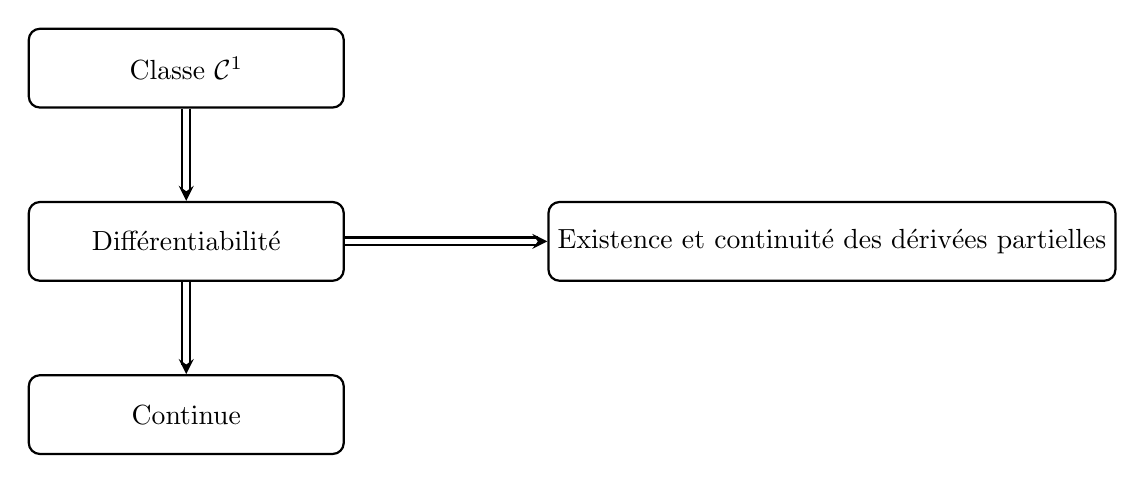
\begin{tikzpicture}[node distance=2.2cm, >=stealth, thick]

        % Styles
        \tikzstyle{node}=[rectangle, draw, rounded corners, align=center, minimum width=4cm, minimum height=1cm]

        % Nœuds
        \node[node] (c1) {Classe $\mathcal{C}^1$}; 
        \node[node, below of=c1] (diff) {Différentiabilité}; 
        \node[node, right of=diff, xshift=6cm] (exists) {Existence et continuité des dérivées partielles}; 
        \node[node, below of=diff] (continue) {Continue}; 

        % Flèches doubles
        \draw[->, double distance=2pt] (c1) -- (diff); 
        \draw[->, double distance=2pt] (diff) -- (exists); 
        \draw[->, double distance=2pt] (diff) -- (continue); 

    \end{tikzpicture}
    }
    \caption{Schéma des implications entre les notions de continuité, différentiabilité et classe $\mathcal{C}^1$.}
    \label{fig:implications_diff}
\end{figure}


\subsection{Formule de Taylor à l'ordre 1}

Essayons maintetant de voir ce que peut nous apporter la différentiaibilité dans le cas d'une fonction 
$f : U \subset \R^2 \longrightarrow \R$ pour laquelle le graphe est représenté en 3 dimensions. 
Supposons que $f$ est de classe $ \mathcal{C}^1$ sur $U$ et soit $ a = (a_1, a_2) \in U$. 
Le graphe de $f$ est donc représenté par : 
    \[ S = \{(x,y,z) \in \R^3 \; | \; f(x,y) = z\} \] 

Or $f$ est \emph{différentiable} donc il existe $V$ un voisinnage de $(0,0) \in \R^2$ et 
$\varepsilon : V \longrightarrow \R$ tels que : 
    \[ \forall h \in \R^2, \quad f(a + h) = f(a) + L(h) + ||h|| \varepsilon (h) \] 
avec $ \varepsilon(h) \underset{h \to (0,0)}{\longrightarrow} 0$. De sorte que pour tout $ (h_1, h_2) = (x - a_1, y -a_2) \in \R^2$, on ait :
    \[ 
        L(h_1, h_2) = \langle \nabla f(a) , h \rangle 
        = \frac{ \partial f}{ \partial x_1}(a) \times h_1 + \frac{ \partial  f}{ \partial x_2}(a) \times h_2 
    \]     
ainsi : 
    \begin{align*}
        & f(a + h) - f(a) = \frac{ \partial f}{ \partial x_1}(a) \times h_1 + \frac{ \partial  f}{ \partial x_2}(a) \times h_2 + ||h|| \varepsilon(h) \\ 
        \Longrightarrow \; & z = f(x, y) = f(a) + \frac{ \partial f}{ \partial x_1}(a) (x - a_1) + \frac{ \partial f}{ \partial x_2}(a) (y - a_2) + ||(x,y) - a|| \varepsilon((x,y) - a) 
    \end{align*}
La différentiabilité de $f$ au point $a$ garantit l'existence d'un plan tangent au graphe de $f$. 

\begin{definition}[Plan Tangent]
    Soit $f : \R^2 \longrightarrow \R$. On appelle plan tangent à la surface $S$ en $a \in \R^2$ d'équation cartésienne 
    $z = f(x,y)$ le plan de $\R^3$ d'équation cartésienne : 
        \[ \boxed{z = f(a) + \frac{ \partial f}{ \partial x_1} (a) (x - a_1) + \frac{ \partial f}{ \partial x_2} (a) (y - a_2) } \] 
\end{definition}

% ==================================================================================================================================
% Propriétés des applications différentiables

\section{Propriétés des applications différentiables}

Maintenant que nous avons vu en quoi consiste la différentiabilité ainsi que ses implications, 
attardons nous sur les propriétés des applications différentiables. 

\subsection{Opérations Algébriques et Différentiabilité}

\begin{prop}[Opérations]
    Soient $f,g : U \subset \R^n \longrightarrow \R^p$ deux applications différentiables 
    en $a \in \U$ et $ \lambda : \R^n \longrightarrow \R$. Soit $\alpha \in \R$. 
    On a les propriétés suivantes : 
    \begin{enumerate}
        \item $f + g$ est diférentiable et : 
            \[ d(f + g)_a = df_a + dg_a \] 
        \item $\lambda f$ est différentiable et : 
            \[ d(\lambda f)_a = d(\lambda)_a f + \lambda df_a \]
        \item Si $\lambda$ ne s'annule pas au voisinnage de $a$, alors $1/\lambda$ est différentiable et : 
            \[ d \left(\frac{1}{\lambda}\right)_a = \frac{- d\lambda_a}{\lambda^2} \] 
        \item si $\lambda$ ne s'annule pas au voisinnage de $a$ on en déduis donc que $f/\lambda$ 
        est différentiable et : 
            \[ d \left(\frac{f}{\lambda}\right)_a = \frac{(df_a)\lambda - (d\lambda_a)f}{\lambda^2} \] 
        \item Si $\lambda$ est strictement positive au voisinnage de $a$ alors $\lambda^\alpha$ 
        est différentiable et : 
            \[ d(\lambda^\alpha)_a = \alpha \lambda^{\alpha - 1} (d\lambda_\alpha) \]
    \end{enumerate}
\end{prop}

\subsection{Différentielle d'une composée : Règle de la chaine}

\subsection{Différentielle d'une réciproque}

\subsection{Théorème d'inversion globale}


% ==================================================================================================================================
% Théorème des accroissements finis

\section{Théorème des accroissements finis}


% ==================================================================================================================================
% Extrema d'une fonction numérique

\section{Extrema d'une fonction numérique}

La fin de ce cours est consacrée à l'utilisation des outils étudiés dans le constexte de 
la recherche d'extrema. 
En effet, en dehors du cadre théorique de ce cours, il peut être utile de déterminer précisément (ou d'approximer)
les extrema d'une fonction de plusieurs variables. C'est notamment le cas lors de l'application 
de l'algorithme de descente de gradient. 

Commençons tout d'abord par définir les objets de ce cours. 

\begin{definition}[Extrema]
    Soit $f : U \subset \R^n \longrightarrow \R$ et $a \in U$. 
    \begin{enumerate}
        \item On dit que $f$ \emph{admet un minimum local en $a$} (resp. local strict) si 
        il existe $\alpha > 0$ tel que : 
            \[ \forall x \in U \cap B(a, \alpha), \quad f(x) \geqslant f(a) \] 
            \[ (\text{resp. } \forall x \in U \cap B(a, \alpha), \quad f(x) > f(a)) \] 
        \item On dit que $f$ \emph{admet un maximim local en $a$} (resp. local strict) si 
        il existe $\alpha > 0$ tel que : 
            \[ \forall x \in U \cap B(a, \alpha), \quad f(x) \leqslant f(a) \] 
            \[ (\text{resp. } \forall x \in U \cap B(a, \alpha), \quad f(x) < f(a)) \] 
        \item On parlera de la même façon de maximum/minimum global. 
    \end{enumerate}
    Pour désigner les maximums/minimums locaux/globaux d'une fonction, on parlera \emph{d'extrema}. 
\end{definition}

\begin{remark}
    Pour faire le lien avec le début de ce cours, on peut remarquer que 
    $f$ présente un extremum local en $a$ si $f(a +h) - f(a)$ est de signe constant sur UN voisinnage de $0_{\R^n}$. 
    Au contraire, $f$ ne présentera pas d'extrema local en $a$ si $f(a + h) - f(a)$ change de signe sur 
    TOUT voisinnage de $0_{\R^n}$. 
\end{remark}

Nous allons tout d'abord chercher à déterminer des conditions nécessaires à la présence d'extrama 
d'un champ de vecteurs quelconques puis nous détaillerons des conditions suffisantes 
dans le cas général, puis dans le cas d'une fonction de deux variables. 

\subsection{Condition Nécessaire}

\begin{theorem}[Existence d'extrema]
    Soit $f : U \subset \R^n \longrightarrow \R$ différentiable sur $U$ ouvert et $a \in U$. 
    Si $f$ présente un extremum local en $a$ alors : 
        \[ df_a = 0 \] 
    i.e 
        \[ \forall i \in \llbracket 1, n \rrbracket, \quad \frac{ \partial f}{ \partial x_i}(a) = 0 \iff \nabla f(a) = 0 \] 
    On appelera ces points des \emph{singuliers}, \emph{critiques} ou \emph{stationnaires}. 
\end{theorem}

Attention, ce n'est pas une condition suffisante ! 

\subsection{Conditions suffisantes : cas général}

\begin{theorem}[Conditions Suffisantes (cas général)]
    Si $a \in U$ est un point critique de $f : U \subset \R^n \longrightarrow \R$ de classe $ \mathcal{C}^2$ sur 
    $U$ alors : 
    \begin{itemize}
        \item Si toutes les valeurs propres de $H_a$ sont strictement positives, alors $f$ présente un
        minimum local strict en $a$. 
        \item Si toutes les valeurs propres de $H_a$ sont strictement négatives, alors $f$ présente un
        maximum local strict en $a$. 
        \item Si $H_a$ admet deux valeurs propres non nulles de signe opposé, alors $f$ admet un point selle en $a$. 
        \item Dans le cas où $0$ est une valeur propre de $H_a$ et que toutes les autres valeurs propres sont 
        de même signe, on ne peut conclure sans une étude approfondie. 
    \end{itemize}
\end{theorem}

\subsection{Conditions Suffisantes : (cas $n = 2$)}

Dans le cas d'une fonction de deux variables, la matrice hessienne de $f$ est de taille 2. 
On peut alors poser : 
    \[ 
        \Delta = rt - s^2    
        \quad \text{où} \quad H_a = 
            \begin{pmatrix}
                r & s \\ 
                s & t 
            \end{pmatrix}
    \] 

On a alors les conditions suivantes : 

\begin{theorem}[Conditions Suffisantes (cas $n = 2$)]
    Soit $f$ une fonction de classe $ \mathcal{C}^2$ sur un ouvert $U$ de $\R^2$ dans $\R$ 
    et $a \in U$ un point critique de $f$. 
    \begin{enumerate}
        \item Si $\Delta > 0$ alors $f$ admet un extremum local strict en $a$ : 
            \begin{itemize}
                \item Si $r > 0$ (ou $t > 0$) c'est un minimum. 
                \item Si $r < 0$ (ou $t < 0$) c'est un maximum. 
            \end{itemize}
        \item Si $\Delta < 0$ alors $f$ n'admet pas d'extrema en $a$, c'est un point selle. 
        \item Si $\Delta = 0$, il faut efectuer une étude plus fine à la main. 
    \end{enumerate}
\end{theorem}


